\section{Haciendo consultas}

En esta sección se ilustrará cómo funciona el algoritmo que utiliza el programa al momento de resolver una consulta.

% Asumo que levantamos la tabla en memoria cada vez que se realiza una consulta. No es lo ideal, pero es lo que pide el enunciado.
\subsection{Puesta en marcha}

\begin{figure}[!ht]
\centering
    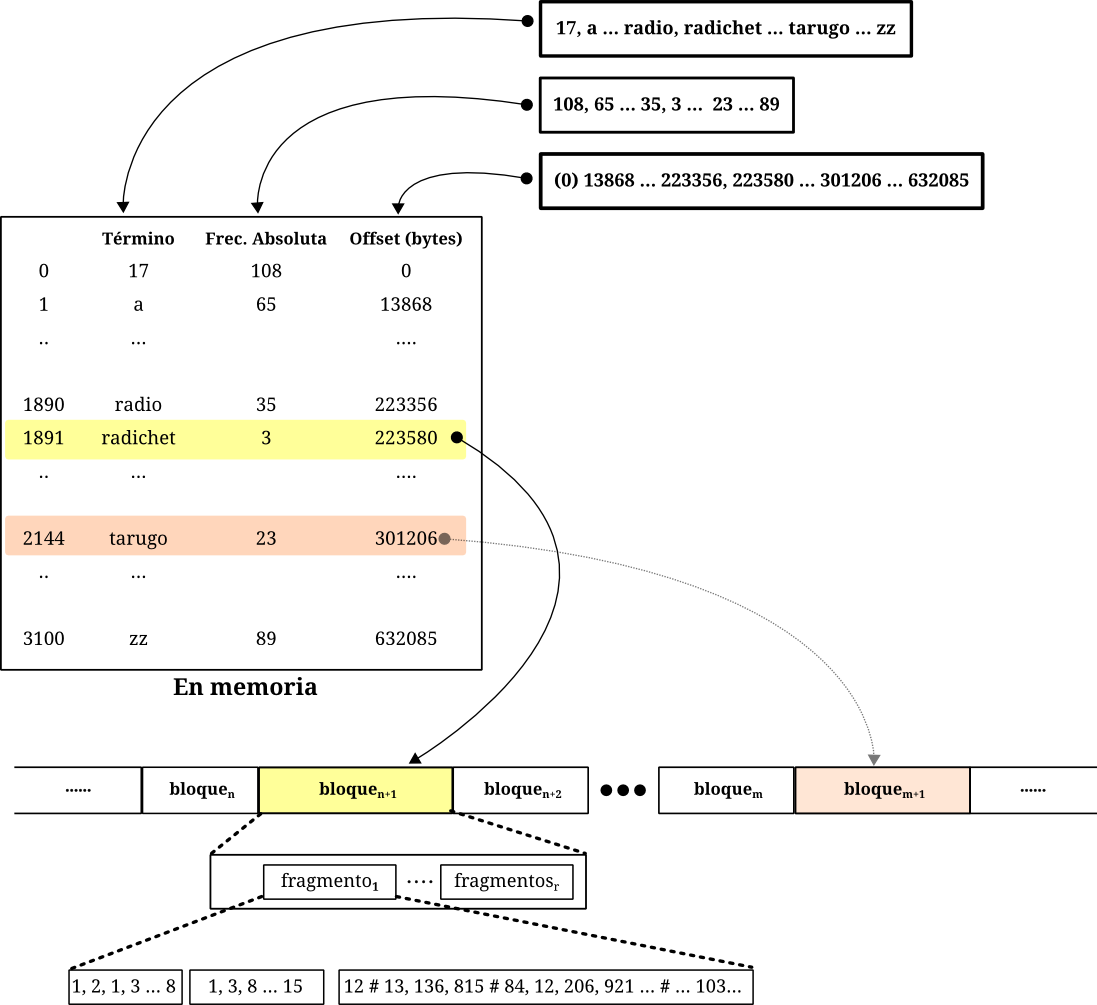
\includegraphics[scale=0.8]{./Images/consulta1.png}
\caption{Armado en memoria de la tabla de términos y búsqueda en el índice invertido}
\label{fig:consulta1}
\end{figure}


Ni bien se ejecuta el programa, éste se prepara para resolver la consulta armando para ello una tabla en memoria. Esta tabla se compondrá de tres columnas: Término, Frecuencia Absoluta y Offset.

Cada columna se extrae descomprimiendo desde disco los archivos .dic, .frq y .ofs respectivamente.
A primera vista, pareciera descabellado cargar el contenido de estos 3 archivos en memoria, pero haciendo algunas cuentas se ve que el espacio ocupado no es intimidante:

Se estima que para una colección de 1 millón de documentos habrá aproximadamente 500000 términos distintos. Si consideramos que en promedio, los términos ocupan 6 bytes aproximadamente. Si además le sumamos a esto 2 bytes por término (contemplando su frecuencia absoluta y su offset), se tiene que se requerirán 8 bytes por término. Haciendo la cuenta: $500000 \times 8$ = 4 millones de Bytes $\approx$ 3906 KBytes $\approx$ \textbf{3.8 MBytes}.

\paragraph{Nota} Lo ideal sería cargar esta tabla en memoria por única vez y luego realizar todas las consultas que se deseen. Pero por restricciones del enunciado del presente trabajo práctico, se cargará la tabla de nuevo para cada consulta.

\subsection{Ejemplo de consulta}

\subsubsection{Normalización y búsqueda}

Supongamos por ejemplo que el usuario ingresó la siguiente frase: <<Radichet, tarugo>>

El primer paso será normalizar la consulta pasando todas las palabras a letra minúscula y eliminando los caracteres que el sistema ignora como son los signos de puntuación. La consulta quedará entonces así: <<radichet tarugo>>
A partir de la consulta normalizada se obtienen los términos <<radichet>> y <<tarugo>>. 
A continuación se los ubica en la tabla generada (ver Figura \ref{fig:consulta1}) y se obtienen sus frecuencias absolutas y offset.


Con el offset, se ubican los bloques que corresponden a cada término en el índice invertido (archivo .idx) y se los descomprime obteniendo los documentos donde aparecen y las posiciones dentro de los mismos como se muestra en la Figura \ref{fig:consulta2}.


\begin{figure}[!ht]
\centering
    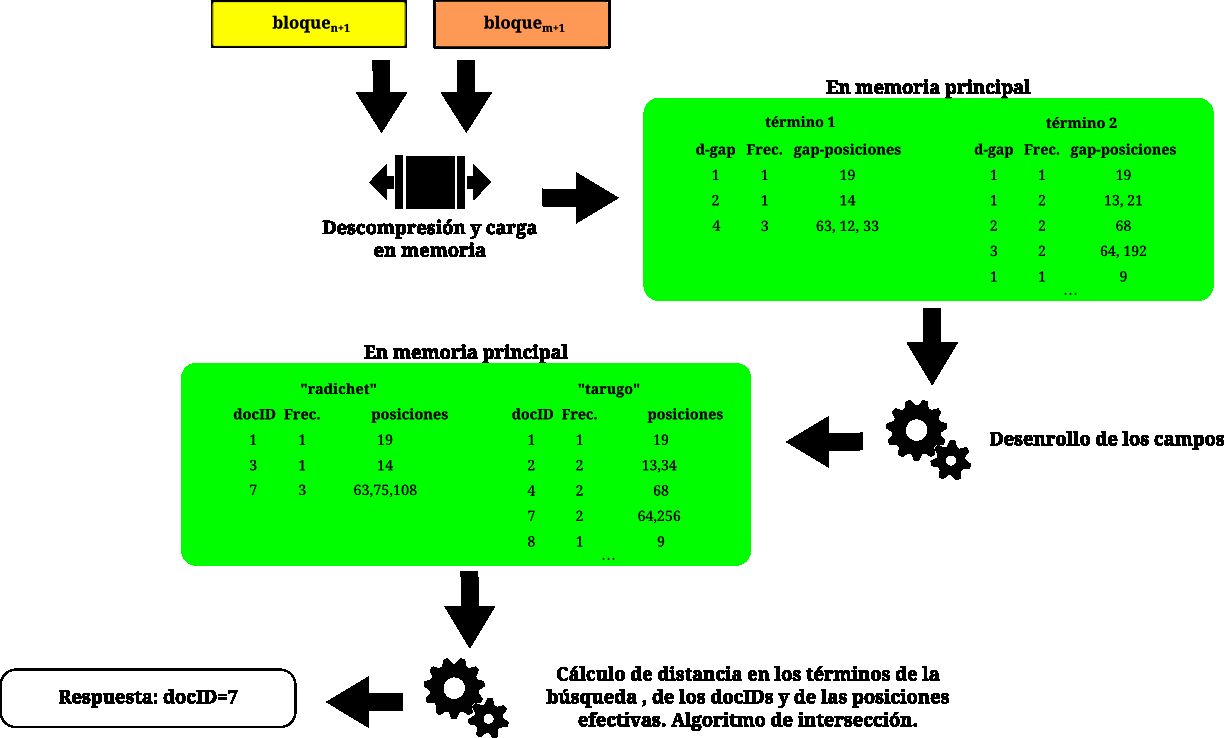
\includegraphics[scale=0.8]{./Images/consulta2.png}
\caption{Obtención de las posiciones a partir de la descompresion de bloques}
\label{fig:consulta2}
\end{figure}


\subsubsection{Algoritmo de intersección}

La consulta de frases implica que la consulta es de tipo booleana, por lo que se la puede ver de la siguiente forma: 
\[ <<radichet>> AND <<tarugo>> \]
Los documentos entregados como resultado de esta consulta serán:
\begin{enumerate}
	\item los que contengan ambos términos y
	\item los que tengan a <<radichet>> en la posición \textit{i} y a <<tarugo>> en \textit{i+1}.
\end{enumerate}

Para resolver el primer punto se utiliza la frecuencia absoluta de los términos (que es la cantidad de documentos en los que aparece cada uno). En el ejemplo, el término <<radichet>> tiene frecuencia 3 y <<tarugo>> 23 por lo que, la máxima cantidad de documentos que podrán cumplir con los requisitos, serán 3. 
Finalmente se ve que solo 2 documentos (el 1 y el 7) contienen a ambos términos).

El segundo punto se resuelve recorriendo la lista de posiciones de los documentos 1 y 7 para cada término en simultaneo.

Finalmente, los documentos que cumplen con los dos puntos son presentados como resultado. En el ejemplo solo el documento de docID $=$ 7 cumple con los requisitos (<<radichet>> en posición 63 y <<tarugo>> en 64).



